\documentclass[a4paper, 12pt]{article}
\usepackage[T1]{fontenc}
\usepackage[utf8]{inputenc}
\usepackage[english]{babel}
\usepackage{mathtools}
\usepackage{amsfonts}
\usepackage{amsmath}
\usepackage{amsthm}
\usepackage{mathrsfs}
\usepackage{enumitem}
\usepackage{booktabs}
\usepackage{array}

% Avoid paragraph indent
\setlength{\parindent}{0pt}
% Useful floor and ceiling functions
\DeclarePairedDelimiter{\floor}{\lfloor}{\rfloor}
\DeclarePairedDelimiter{\ceil}{\lceil}{\rceil}
% Argmax/Argmin notation
\DeclareMathOperator*{\argmax}{argmax} 
\DeclareMathOperator*{\argmin}{argmin}
\DeclareMathOperator*{\rep}{rep} 
% Modified margins
\usepackage[margin=2cm]{geometry}
% This avoids hypenation
\hyphenpenalty=1000
\usepackage{tikz}
\usetikzlibrary{arrows,calc,positioning,shadows,shapes}
\usepackage{graphicx}
\usepackage{subfig}
\graphicspath{{./images/}}
\captionsetup[figure]{labelfont={bf},name={Figure},labelsep=period}
\captionsetup[table]{labelfont={bf},name={Table},labelsep=period}

\usepackage{float}
\usepackage{xfrac}
\usepackage{pgfplots}
\usepackage{titling}
\usepackage[bottom]{footmisc}

%\setlength{\droptitle}{-5em}

\begin{document}

\begin{titlepage}

%\addtolength{\voffset}{-1.3cm}	

\vspace*{1cm}

\begin{center}
\large \textsc{Università degli Studi di Padova \\ Department of Information Engineering}

\vspace*{1cm}

\rule{\linewidth}{1pt} \Huge{ \textsc{Digital Forensics}} \\ {\textsc{Second Laboratory Report}} \rule{\linewidth}{2pt}

\vspace*{1cm}

\large \textsc{Faccin Dario} \\
\normalsize \textsc{ID Number: 1177736}

\end{center}

\section*{Abstract}
Digital visual media represent nowadays one of the principal means for
communication. Lately, the reliability of digital visual information has been questioned,
due to the ease in counterfeiting both its origin and content. Digital image forensics is a research field which aims at validating the authenticity of images by recovering
information about their history.\\
The main problem addressed in this report is the identification of the
imaging device that captured the image.
\end{titlepage}

\section*{Source identification}
\subsection*{Image acquisition process}
The light enters the imaging device through a system of optical lenses, which conveys it towards the imaging sensor. The imaging sensor is the heart of every digital camera, and it is composed of an array of photo detectors, each corresponding to a pixel of the final image, which transform the incoming light intensity into a proportional voltage. Most cameras use CCD (Charged Coupled Device) sensors, but CMOS (Complementary Metal Oxide Semiconductor) imagers can also be found. To render color, before reaching the sensor the light is filtered
by the Color Filter Array (CFA), a specific color mosaic that permits to each pixel to gather
only one particular light wavelength (i.e. color). The CFA pattern arrangement depends on
the manufacturer, although Bayer’s filter mosaic is often preferred. As a result, the sensor
output is a mosaic of e.g. red, green and blue pixels arranged on a single layer. To obtain
the canonical 3-channels representation, the signal needs to be interpolated. Demosaicing
algorithms are applied to this purpose; the missing pixel values in each layer are estimated
based on the values of existing neighbors. Before the eventual storage, additional
processing is performed, such as white balance, gamma correction, and image enhancement.
Finally, the image is recorded in the memory device. The following Figure [\ref{fig:imacq}] illustrates schematically the image acquisition process.

\begin{figure}[H]
	\centering
	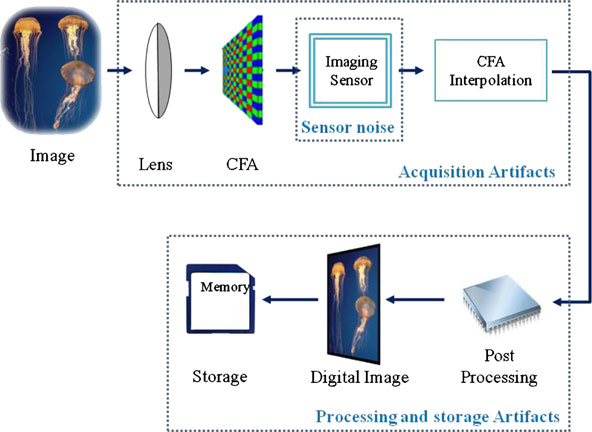
\includegraphics[width=0.5\textwidth]{imageacq}
	\caption{Image acquisition pipeline.}
	\label{fig:imacq}
\end{figure}

\subsection*{Camera identification}
The described image acquisition pipeline is common for most of the commercially
available devices. Each step is performed according to specific manufacturer
choices and hence might depend on the camera brand and model. This variation can be
used to determine the type of camera from which a specific image was obtained. Indeed,
each stage in the pipeline can introduce imperfections in the final image or characteristic
traits: lens distortion, chromatic aberration, pixel defects or CCD sensor imperfections,
statistical dependencies related to proprietary CFA interpolation algorithms and other
intrinsic image regularities. These artifacts are statistically
stable and can be considered as a signature of the camera type or even of the individual
device.

\section*{Sensor imperfections}
Imaging sensors have been shown to introduce various defects and to create noise in the
pixel values. The sensor noise is the result of three main components, i.e. pixel defects,
\textit{Fixed Pattern Noise} (FPN), and \textit{Photo Response Non Uniformity} (PRNU).\\
Pixel defects include point defects, hot point defects, dead pixels, pixel traps, and cluster
defects, which reasonably vary across different sensors, independent on the specific camera
model.\\
FPN and PNRU are the two components of the so-called pattern noise, and depend on
dark currents in the sensor and pixel non-uniformities, respectively. Hence, they are
independent on the image content but closely related to the physical characteristics of each
single sensor. The pattern noise extracted from images taken by the same camera are more
correlated than those extracted from different cameras.
\subsection*{Photo Response Non Uniformity}
Photo Response Non Uniformity (PRNU) is caused by the different sensitivity of the sensors to the light. This behavior is due to the manufacturing process and does not depend on the external temperature or acquisition time.\\
The resulting image can be described as following:
\begin{equation}
\mathbf{I} = \mathbf{I}^{(0)} + \mathbf{I}^{(0)} \mathbf{K} + \mathbf{\Theta}
\end{equation}
where $\mathbf{I}^{(0)}$ is the ideal sensor output (without noise), $\mathbf{K}$ is the PRNU fingerprint of the camera and $\mathbf{\Theta}$ accounts for all the other types of noise.\\
Pattern noise can be estimated by taking the difference between an image $\mathbf{I}$ and its denoised version:
\begin{equation}\label{eq:imdiff}
\mathbf{W_I} = \mathbf{I}- F\left(\mathbf{I}^{(0)}\right)
\end{equation}
where $\mathbf{W_I}$ is called \textit{residual noise} and $F$ is a \textit{denoising filter}.

\subsection*{PRNU fingerprint estimation}
Let $ \mathbf{\hat{I}}^{(0)}$ be the denoised version of $\mathbf{I}^{(0)}$.\\
We can rewrite Equation (\ref{eq:imdiff}) as:
\begin{align}
\mathbf{W_I} & = \mathbf{I}- \mathbf{\hat{I}}^{(0)} \nonumber \\
& = \mathbf{I}- \mathbf{\hat{I}}^{(0)} + \mathbf{I} \mathbf{K} - \mathbf{I} \mathbf{K} \nonumber \\
& = \mathbf{I} \mathbf{K} + \mathbf{I}^{(0)} - \mathbf{\hat{I}}^{(0)} + \left( \mathbf{I}^{(0)}-\mathbf{I} \right) \mathbf{K} + \mathbf{\Theta}
\end{align}
Now let $\mathbf{\Sigma} = \mathbf{I}^{(0)} - \mathbf{\hat{I}}^{(0)} + \left( \mathbf{I}^{(0)}-\mathbf{I} \right) \mathbf{K} + \mathbf{\Theta}$ be the noise independent from $\mathbf{IK}$. We can finally write:
\begin{equation}
\mathbf{W_I} = \mathbf{I} \mathbf{K} + \mathbf{\Sigma}
\end{equation}
Due to the random components related a specific image, the reference PNRU factor $\mathbf{\hat{K}}$ for a particular camera C is obtained can be estimated through Maximum Likelihood.
Given $N$ images $\mathbf{I}_1, \dots, \mathbf{I}_N$, we can reasonably assume that $\mathbf{\Sigma}[i]_1, \dots, \mathbf{\Sigma}[i]_N$ for each pixel $i$ are white Gaussian noise with variance $\sigma^2$. The energy of the PRNU $\mathbf{I} \mathbf{K}$ is small compared to the noise term $\Theta$, so we can also assume that $\mathbf{\Sigma}$ is independent of $\mathbf{I} \mathbf{K}$.\\
For each $i=1,\dots,N$ we have
\begin{equation*}
\dfrac{\mathbf{W}_i}{\mathbf{I}_i} = \mathbf{K} + \dfrac{\mathbf{\Sigma}_i}{\mathbf{I}_k}
\end{equation*}
The log-likelihood of observing $\dfrac{\mathbf{W}_i}{\mathbf{I}_i}$ given $\mathbf{K}$ is
\begin{equation}
L(\mathbf{K}) =-\dfrac{N}{2} \sum_{i=1}^{N}\log\left( \dfrac{2\pi\sigma^{2}}{({\bf I}_{i})^{2}}\right)-\sum_{i=1}^{N}{ \frac{\left(\dfrac{{\bf W}_{i}}{{\mathbf I}_{i}-{\bf K}}\right)^{2}}{\dfrac{2\sigma^{2}}{({\mathbf I}_{i})^{2}}}}
\end{equation}
The estimate is then obtained by computing the first order derivate of $L(\mathbf{K})$ with respect to $\mathbf{K}$ and solving for $\mathbf{K}$:
\begin{equation*}
\dfrac{\partial L(\mathbf{K})}{\partial{\bf K}} = 0 \implies \mathbf{\hat{K}} = \dfrac{\sum\limits_{i=1}^{N} \mathbf{W}_i \mathbf{I}_i}{\sum\limits_{i=1}^{N} \left( \mathbf{I}_i \right) ^2}
\end{equation*}
Computing the second order derivative is useful to obtain the Cramer-Rao lower bound and to infer what are the best images for the PRNU estimation.

\begin{equation}
\dfrac{ \partial^2 L(\mathbf{K})}{\partial \mathbf{K}^2} = \dfrac{\sigma^2}{\sum\limits_{i=1}^{N} \left( \mathbf{I}_i \right) ^2}
\end{equation}

The luminance $\mathbf{I}_i$ should be as high as possible but not saturated, since saturated pixels carry no information on the PRNU factor.\\
Also $\text{var}(\mathbf{\hat{K}}) \sim \sigma^2$, therefore better estimates are obtained using smooth test images.

\subsection*{PRNU fingerprint detection}

\section*{Results}

The \textsc{Matlab} code provided for this assignment performs the CONTINUA.\\
Among the returned values, the most important are the \textit{Peak-to-Correlation Energy} (PCE) and the \textit{Probability of False Alarm} (P\_FA).\\
The Peak-to-Correlation Energy is a measure of ...\\
Probability of False Alarm is a measure of 


\begin{figure}[H]
	\centering
	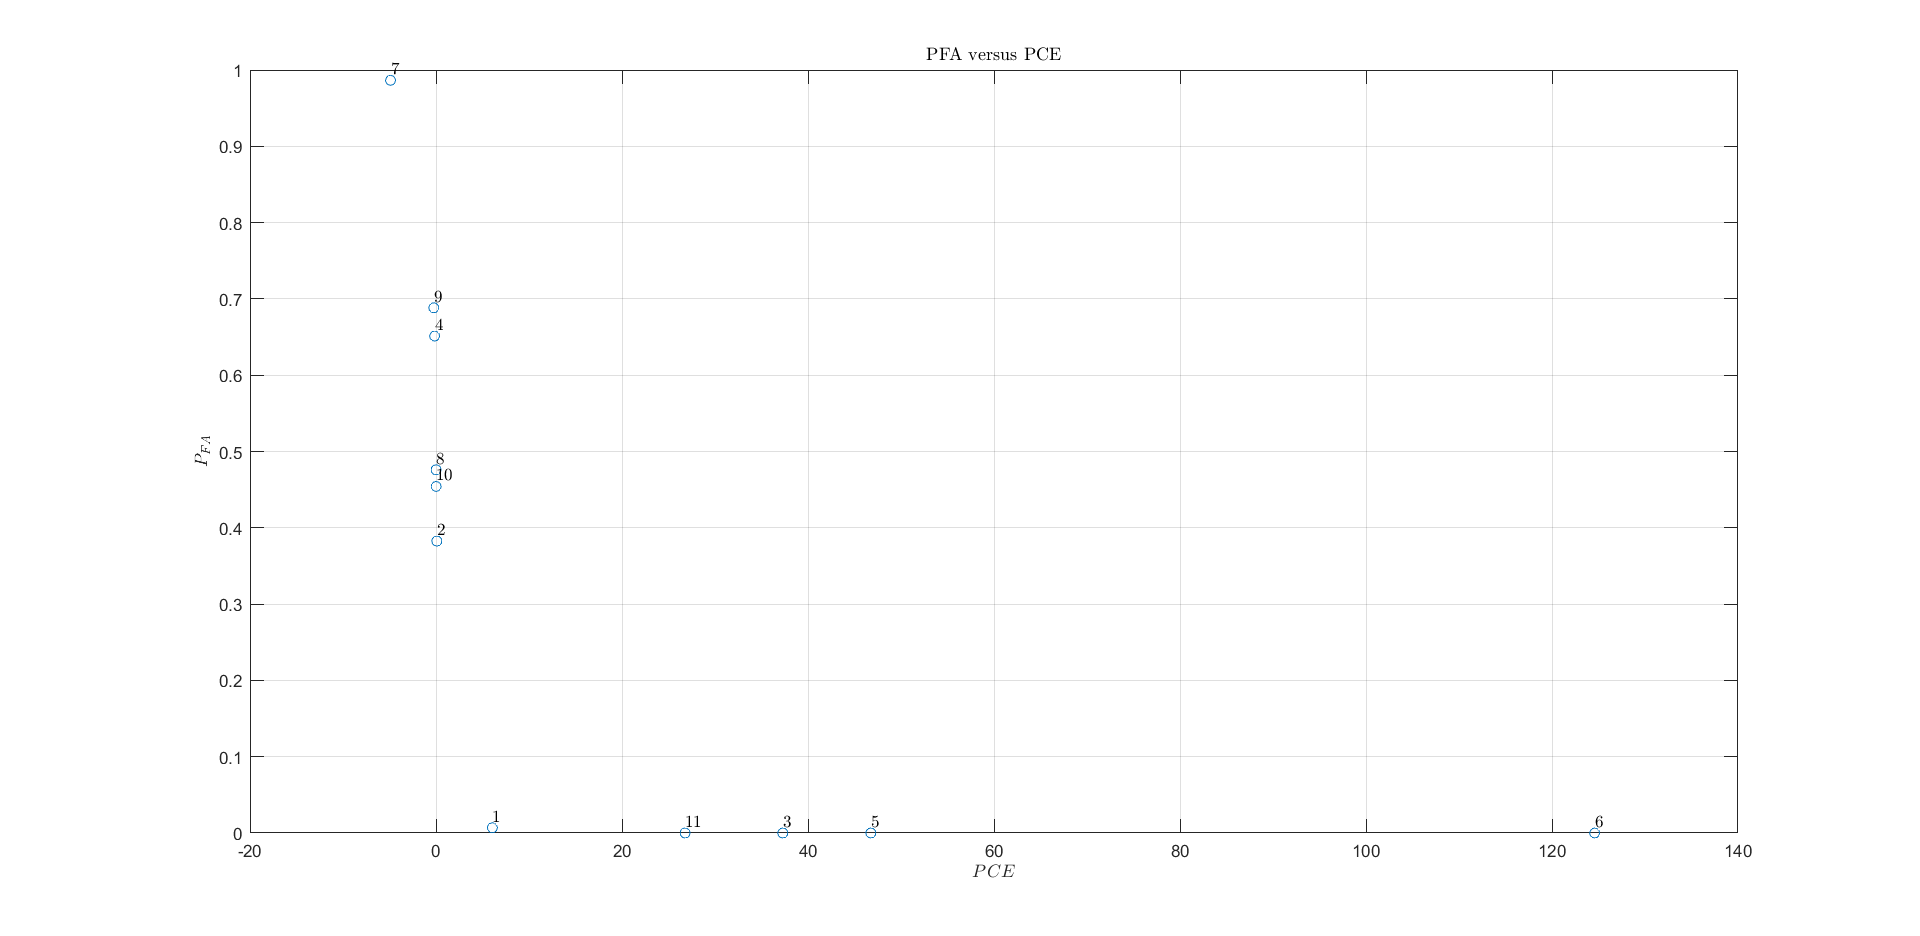
\includegraphics[width=0.7\textwidth]{defaultdataset}
	\caption{Results obtained for the default data set.}
	\label{fig:defaultdataset}
\end{figure}

From Figure [\ref{fig:defaultdataset}] it is possible to see which

\begin{thebibliography}{3}
	\bibitem{dig}
	Dugelay J., Redi J., Taktak W.
	\textit{Digital image forensics}.
	2010.
	
	\bibitem{golomb}
	Milani S.,
	\textit{Digital Forensics: course lectures}.
	2018.
\end{thebibliography}

\end{document}